\documentclass{article}
\usepackage[utf8]{inputenc}

\usepackage{tikz}
\usetikzlibrary{positioning, fit}

\usepackage{skak}

\begin{document}

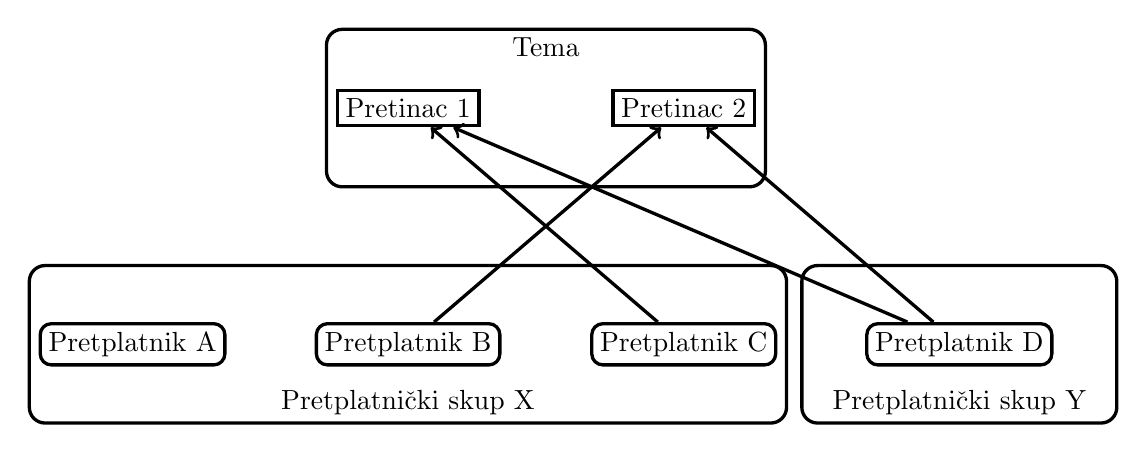
\begin{tikzpicture}[ % has a lot of options; consult the pgf manual
bend angle=45,
long_square/.style={rectangle, draw=black, fill=white, very thick, inner sep=3pt, minimum width=14mm},
rounded_square/.style={rectangle, rounded corners, draw=black, fill=white, very thick, inner sep=3pt, minimum width=14mm},
empty_circle/.style={rectangle, rounded corners=2mm, draw=black, fill=white, very thick, minimum size=4mm},
point/.style={circle, inner sep=0mm},
fit_square/.style={rectangle, rounded corners=2mm, draw=black, very thick, minimum height=20mm},
both_arrow/.style={<->, very thick},
out_arrow/.style={->, very thick},
in_arrow/.style={<-, very thick},
above_edge_text/.style={above, midway, sloped}
]

\node[long_square](partition_1) at (3.5,0) {\king Pretinac 1};
\node[long_square](partition_2) at (7,0) {\king Pretinac 2};

\node[rounded_square](consumer_1) at (0,-3) {Pretplatnik A};
\node[rounded_square](consumer_2) at (3.5,-3) {Pretplatnik B};
\node[rounded_square](consumer_3) at (7,-3) {Pretplatnik C};
\node[rounded_square](consumer_4) at (10.5,-3) {Pretplatnik D};

\node[fit_square, fit=(partition_1) (partition_2)] (topic) {};
\node[anchor=north] at (topic.north) {Tema};

\node[fit_square, fit=(consumer_1) (consumer_2) (consumer_3)] (group_1) {};
\node[anchor=south] at (group_1.south) {Pretplatnički skup X};

\node[fit_square, minimum width=40mm, fit=(consumer_4)] (group_2) {};
\node[anchor=south] at (group_2.south) {Pretplatnički skup Y};



\draw[out_arrow](consumer_2) to [] node[auto]{} (partition_2);
\draw[out_arrow](consumer_3) to [] node[auto]{} (partition_1);

\draw[out_arrow](consumer_4) to [] node[auto]{} (partition_1);
\draw[out_arrow](consumer_4) to [] node[auto]{} (partition_2);

\end{tikzpicture}

\end{document}